\chapter{Lecture 19 - Natural Circulation}
\label{ch:ch19}
\section{Objectives}
The objectives of this lecture are:
\begin{enumerate}
\item Describe natural circulation 
\item Demonstrate an analysis of natural circulation flow for the NucScale SMR
\item Discuss the advantages and disadvantages of natural circulation for nuclear power reactors.
\end{enumerate}

\section{Motivation}
The possibility that, at any given time for any of a number of reasons, pumps providing cooling flow to the core may lose power is a major contributor to the overall probability of core damage for nuclear reactors. If electrical power is lost to cooling pumps for a PWR, for instance, an operator may take action to restore flow; or they may not.  Wouldn't it be a lot better and more safe if cooling flow circulation would take place \emph{without any pumps at all} and there would be no need for operators to take actions in the event of loss of power; indeed, there may not be a need for any \emph{operators} or \emph{electrical power} at all!  This is the motivation for natural circulation for primary coolant flow.  

\section{Natural Circulation} \index{natural circulation}

In principle, only three conditions are required to achieve natural circulation:

\begin{enumerate}
\item A heat sink and a heat source
\item The heat source must be ``below'' the heat sink with respect to some gravitational reference; and
\item flow-paths must exist for the fluid to flow and carry energy to and from the heat source and heat sink.
\end{enumerate}
A schematic representation is provided in Figure \ref{fig:nat_circ}.  The hydraulic pressure, providing the driving force for natural circulation is given by:
$$\text{Driving Force} = \left(\rho_c - \rho_h \right) \frac{g}{g_c}h $$
where $\rho_c$ and $\rho_h$ are the density of the cold and hot fluids respectively; $g$ is the acceleration due to gravity; $g_c$ is that annoying constant we have to include from time-to-time when using USCS units; and $h$ is the height of the heat sink relative to the heat source.
\begin{marginfigure}
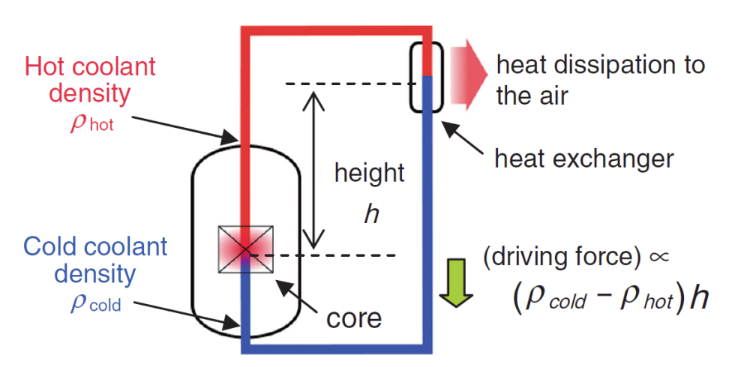
\includegraphics{nat_circ.png}
\caption{Schematic representation of a minimal natural circulation arrangement}
\label{fig:nat_circ}
\end{marginfigure}

\newthought{The driving force} will establish natural circulation flow.  The hydraulic pressure drop from major and minor head losses constitute the resistance to flow:
$$\text{Flow Resistance} = \left(\frac{fL}{D} + \Sigma K \right) \rho \frac{g}{g_c}\frac{v^2}{2g} $$
If velocity $(v)$ is zero, there is no resistance and flow will commence. As velocity goes up, flow resistance increases.  Velocity will continue to increase until the flow resistance is in equilibrium to the driving force.  Since the driving force is created by the density, and thus temperature difference between the hot and cold columns of water, the equilibrium velocity is a function of the thermal power output of the heat source. 

\section{NuScale Natural Circulation Demonstration} \index{NuScale reactor}
\begin{marginfigure}
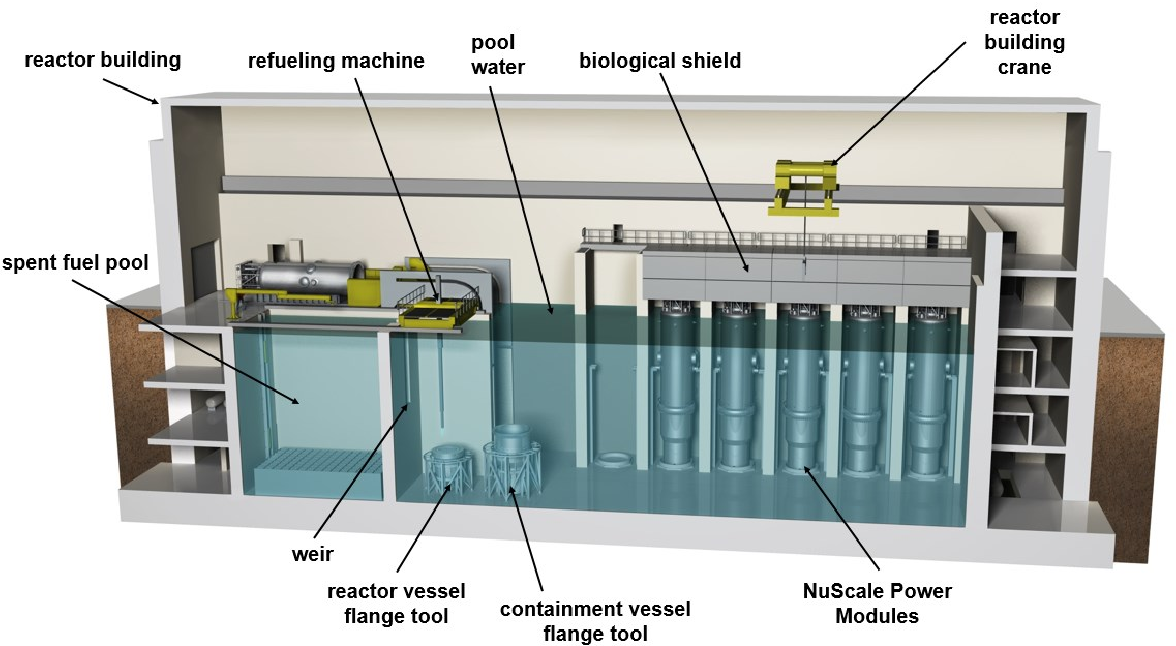
\includegraphics{nuscale_power_building.png}
\caption{NuScale reactor containment building.}
\label{fig:nuscale_power_building}
\end{marginfigure}
\index{integral reactor}
A current reactor concept design that depends upon natural circulation for primary coolant flow is the NuScale reactor.  The NuScale concept includes a collection of power modules contained within an underground pool-type containment building as in Figure \ref{fig:nuscale_power_building}.  Each individual power module is a pressurized water reactor of \emph{integral} design.\marginnote{\textbf{Integral} pressurized water reactors combine the reactor core, steam generator, and pressurizer within a single pressure vessel.} Primary coolant flow within each power module is driven by natural circulation; a simplified schematic to illustrate the flow-paths is shown in Figure \ref{fig:nuscale_schematic}.    
\begin{marginfigure}
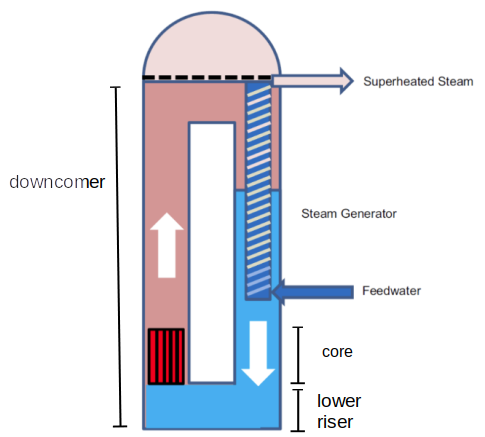
\includegraphics{nuscale_schematic.png}
\caption{Schematic of natural ciruclation in a NuScale power module.}
\label{fig:nuscale_schematic}
\end{marginfigure}
To enable a quantitative analysis, we will estimate some of the dimensions:
\begin{itemize}
\item height of ``downcomer'' - 46 ft
\item height of the ``lower riser'' - 9.4 ft
\item height of the core - 7.9 ft
\end{itemize}
We combine these to estimate the height of the thermal driving head $(H)$:
$$H = L_{\text{downcomer}} - L_{\text{lower riser}} - L_{\text{core}}$$
For the thermal model of the core, we will make the following simplifications:
\begin{itemize}
\item The core $\Delta T$, which is $T_H - T_C$ is dictated by core power and coolant mass flow rate.
\item We will assume average coolant temperature remains constant
\end{itemize}
The thermal driving head will thus be computed as:
$$\Delta P_{\text{thermal}} = \left(\rho_C - \rho_H \right)\frac{g}{g_c} H $$
Rather than explicitly creating a hydraulic model of the core and natural circulation flow path, we will assume that the coefficients comprising major and minor head losses, $\frac{fL}{D} + \sum{K}$, are constant $(C)$.  Therefore the hydraulic flow resistance will be given by:
$$\Delta P_{\text{hydraulic}} = C \times \rho \frac{v^2}{2 g_c}$$
where $\rho$ is the nominal density at the average coolant temperature.  The mass flow rate from natural circulation will thus be: 
$$\dot{m} = \rho v \text{A}_{\text{flow}}$$
where $\text{A}_{\text{flow}}$ is the total core flow area.  A complete MATLAB code for this analysis is provided in the appendices.  The resulting mass flow rate is shown in Figure \ref{fig:NuScale_NC_Plot}.
\begin{marginfigure}
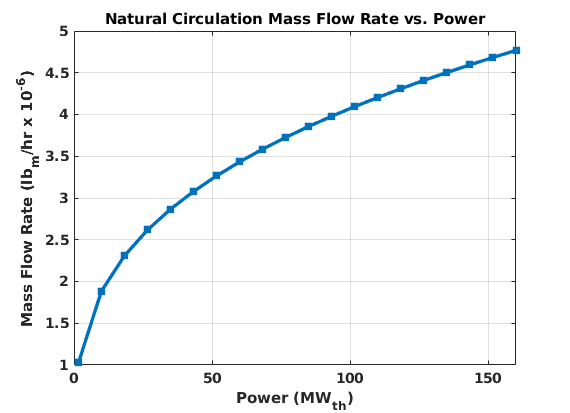
\includegraphics{NuScale_NC_Plot.png}
\caption{Natural Circulation mass flow rate as a function of reactor power for a simplified NuScale power module.}
\label{fig:NuScale_NC_Plot}
\end{marginfigure}

\section{Advantages and Disadvantages of Natural Circulation}
Some advantages of natural circulation include:
\begin{enumerate}
\item Natural circulation eliminates dependence on pumps for coolant circulation. Pumps are problematic in that they:
\begin{enumerate}
\item require electrical power (that may fail);
\item are subject to mechanical failure; and
\item require space along with mechanial and electrical connections.  This is particularly a disadvantage for integral reactor designs
\end{enumerate}
\item does not require human action to maintain flow; and
\item for some applications---such as propulsion for a military submarine---natural circulation is generally more quiet than forced circulation with a centrifugal pump
\end{enumerate}

Some disadvantages of natural circulation include:
\begin{enumerate}
\item limited control over flow rate.  The thermal/hydraulic design is constrained and dependence on flow from natural circulation may limit the thermal power density that can safely be achieved.
\item the thermal driving head for natural circulation depends upon coolant density difference which, in turn, is a function of coolant temperature difference across the core.  A need to increase thermal driving head may result in unacceptably high differential temperatures and thermal stress for mechanical components in the core.
\item the procedures for establishing natural circulation flow may involve complexities and there may be no simple way to rapidly change coolant flow rate should the need arise.
\end{enumerate}

The potential for safety and reliability that can come from natural circulation is the main source of interest.

\section{Summary}
Students are strongly encouraged to carefully work through the MATLAB demonstration code provided in the appendix.  Analyze the parameters and make changes to the model to be sure you understand what is going on.  One thing you may notice is the importance of the \emph{distance} between the hot- and cold-temperature reservoirs.  The greater that distance, the greater thermal driving head will be for a given temperature differential.  This is one reason why the NuScale modules are relatively ``tall and skinny'' compared to a typical PWR pressure vessel---beyond the need to simply make space for the steam generator and pressurizer within the integral design.  

The Economically Simplified Boiling Water Reactor (ESBWR) also relies on natural circulation in lieu of recirculation pumps for reactivity control.\cite{hinds2006next}  The pressure vessel for the ESBWR is correspondingly much taller than that of a typical BWR, in part, to provide greater driving head for natural coolant circulation. 

Even if a reactor uses pumps or compressors to drive coolant circulation, natural circulation is still relevant for the engineering design analysis.  Nearly all pressurized water reactors have emergency cooling systems incorporated into their design for use in the event of primary coolant system failure.  It is very common for these emergency cooling systems to utilize natural circulation.  

